\documentclass[12pt]{report}
\usepackage{flushend}
\usepackage{graphicx}
\usepackage[noadjust]{cite}
\usepackage[toc,acronym,sort=def]{glossaries}
\usepackage{sectsty}
\usepackage{setspace}
\usepackage{enumerate}
\usepackage{IEEEtrantools}
\usepackage{paralist}
\usepackage{chngcntr}
\usepackage{ftnxtra}
\usepackage{amsmath}
\usepackage{amssymb}
\usepackage{algorithm}
\usepackage[noend]{algpseudocode}
\usepackage{booktabs}
\usepackage{longtable}
\usepackage{array}
\usepackage{tabularx}
\usepackage{float}
\usepackage{subcaption}
\usepackage{multirow}
\usepackage{textcomp}
\usepackage{url}
\counterwithout{footnote}{chapter}
%\usepackage[top=1.4 in]{geometry}
\algnewcommand{\LeftComment}[1]{\Statex \(\triangleright\) #1}
\renewcommand{\bibname}{References}
\renewcommand{\algorithmicrequire}{\textbf{Input:}}
\renewcommand{\algorithmicensure}{\textbf{Output:}}
\chapterfont{\centering}
\pagestyle{headings}
\onehalfspacing

%************Glossary*************%

\makeglossaries

\newglossaryentry{dna}
{
    name=DNA,
    description={Deoxyribo Nucleic Acid, a molecule that codes genetic instructions in living organisms. It is a \emph{string} of 4 `nucleotides' - Nitrogen containing bases: Cytosine (C), Guanine (G), Adenine (A), and Thymine (T)}
}

%********End of Glossary**********%

\begin{document}

\begin{titlepage}
\begin{center}
\vspace{1cm}
\huge
\textbf{Medical Diagnosis and Report Generation for Endoscopic Procedures Using Vision-Language Models}\\

\normalsize
\vspace{1cm}
\emph{Submitted by}\\
\vspace{0.5cm}
\begin{tabular}{ll}
\textbf{Praval Pattam} & \textbf{Affil.: B220057CS}\\
\textbf{Theenesh Potluri} & \textbf{Affil.: B221121CS}\\
\textbf{Pranav Sai Sarvepalli} & \textbf{Affil.: B220055CS}\\
\end{tabular}\\
\vspace{0.8cm}
\textbf{Under the Guidance of: Jayaraj PB, Srinivasa TM}\\
\vspace{0.8cm}
\begin{center}
\IfFileExists{nitc-logo.png}{
\includegraphics[width=0.2\textwidth]{nitc-logo.png}}{}
\end{center}
\vspace{0.8cm}
\textbf{Department of Computer Science and Engineering}\\
\textbf{National Institute of Technology Calicut}\\
\textbf{Calicut, Kerala, India - 673 601}\\
\vspace{0.8cm}
\textbf{May 13, 2026}
\end{center}
\end{titlepage}
\pagenumbering{roman}
\begin{spacing}{1.01}
{
\thispagestyle{empty}

\fontsize{14}{14}\selectfont
\centering{\MakeUppercase{\textbf{National Institute of Technology Calicut, Kerala, India - 673 601}}} \\
\vspace*{0.5cm}
\fontsize{12}{12}\selectfont
\centering{\MakeUppercase{\textbf{Department of Computer Science and Engineering}}} \\
\begin{figure}[ht]
{\centering {\IfFileExists{nitc-logo.png}{
\includegraphics[width=0.2\textwidth]{nitc-logo.png}}{}}\par}
\end{figure}
2025\\
\vspace{0.5cm}
\fontsize{14}{14}\selectfont
\textbf{\centering{CERTIFICATE}}\\
\vspace{0.25cm}
\fontsize{12}{12}\selectfont
\onehalfspacing{\textit{Certified that this is a bonafide record of the project work titled}}\\
\vspace*{0.25cm}
\textbf{\MakeUppercase{Medical Diagnosis and Report Generation for Endoscopic Procedures Using Vision-Language Models}}\\
\vspace*{0.25cm}
\onehalfspacing{\centering{\textit{done by}}}\\
\vspace*{0.25cm}
\begin{tabular}{c}
\textbf{Praval Pattam}\\
\textbf{Theenesh Potluri}\\
\textbf{Pranav Sai Sarvepalli}\\
\end{tabular}\\
\vspace*{0.25cm}
\onehalfspacing{ \textit{\centering{of eighth semester B. Tech in partial fulfillment of the requirements for the award of the degree of Bachelor of Technology in Computer Science and Engineering of the National Institute of Technology Calicut}}}\\
\vspace*{0.75cm}
\noindent{
\begin{tabular}{p{6.5cm}p{5.5cm}}
\textbf{Project Guides} & \textbf{Head of Department} \\[2.5cm]
\textbf{Jayaraj PB} \newline Associate Professor &
\textbf{Dr. Subashini R} \newline Associate Professor \\[2.5cm]
\textbf{Srinivasa TM} \newline Assistant Professor & \\
\end{tabular}
}
}
\chapter*{DECLARATION}
We hereby declare that the project titled, \textbf{Medical Diagnosis and Report Generation for Endoscopic Procedures Using Vision-Language Models}, is our own work and that, to the best of our knowledge and belief, it contains no material previously published or written by another person nor material which has been accepted for the award of any other degree or diploma of the university or any other institute of higher learning, except where due acknowledgement and reference has been made in the text.\\

\vspace{2cm}
\noindent{
\begin{tabular}{p{8cm}p{6cm}}
Place :  & Signature : \\
Date : & Name : \\
 & Reg. No. : 
\end{tabular}
}
\newpage 

\begin{abstract}
Background and Objective: Writing endoscopic image reports requires extensive domain expertise, and even experienced clinicians spend substantial time on them. Although multimodal large language models (MLLMs) excel at cross-modal understanding and generation, general models struggle with specialized terminologies, pathological features, and complex medical logic, limiting their accuracy and applicability in endoscopy. Existing fine-tuning methods can improve model performance to some extent, but they often suffer from limited adaptability and insufficient domain-specific knowledge when applied to tasks in specialized fields. Methods: We propose a Multimodal Vision-Language Model for Endoscopic Report Generation (MVLMERG). We apply a two-stage P-LoRA strategy: the first stage infuses domain knowledge from publicly available medical datasets, and the second stage fine-tunes on physician-annotated clinical data to align the model with professional endoscopic reporting conventions. Results: Experimental results show that MVLMERG attains state-of-the-art performance on our custom endoscopic dataset, outperforming all baseline models across all automated evaluation metrics.
\end{abstract}
\chapter*{\rm \large \bf ACKNOWLEDGEMENT}
\vspace{4.0mm}
This work is supported by Department of Computer Science and Engineering, National Institute of Technology Calicut .
\tableofcontents
\addtocontents{toc}{\vskip-30pt}
\end{spacing}
\listoffigures
\listoftables
\vspace{-2 em}
\printglossary[nonumberlist]


\pagenumbering{arabic}

\chapter{Introduction}
\section*{Project Information}
\textbf{Title:} Medical Diagnosis and Report Generation for Endoscopic Procedures Using Vision-Language Models.\\
\textbf{Authors:} Praval Pattam\textsuperscript{B220057CS}, Theenesh Potluri\textsuperscript{B221121CS}, Pranav Sai Sarvepalli\textsuperscript{B220055CS}.\\
\textbf{Affiliations:}\\
Department of Computer Science and Engineering, National Institute of Technology Calicut, Calicut, Kerala, India - 673 601.\\
\textbf{Keywords:} Multimodality; Large language models; Fine-tuning; Vision-language models; Endoscopic report generation.\\

\section{Introduction}
Recent studies have made notable contributions to endoscopic tasks [1,2]. In the medical field, especially in endoscopic examinations, generating high-quality reports is critical for early disease detection, diagnosis, and treatment [3,4]. Endoscopy produces a large amount of image data, which doctors must carefully analyze to write accurate reports. By learning general knowledge from large-scale data, MLLMs can quickly adapt to specific domains and handle the complex mapping between endoscopic images and diagnostic reports [5].
Previous studies [6,7] have focused on building comprehensive multimodal models for medical applications, aiming to achieve integrated reasoning capabilities across modalities. Large-scale medical datasets like PubMed [8] provide abundant general medical knowledge but lack detailed annotations for specific diseases or organs. High-quality annotated endoscopic images are especially scarce, limiting the development of effective diagnostic models. Moreover, training multimodal large models from scratch requires vast computational resources. Thus, efficient fine-tuning of existing large models has become a more practical approach [9].
Although LoRA has demonstrated strong generalizability across various tasks, its fine-tuning performance on specialized downstream tasks still leaves room for improvement [11]. Therefore, effectively leveraging prompt-based methods to enhance LoRA's capability in LLaVA-4 for specialized tasks remains a critical challenge.
In this report, we propose a Multimodal Vision-Language Model for Endoscopic Report Generation (MVLMERG), which achieves state-of-the-art performance in comparisons with mainstream foundational models. To enhance the fine-tuning results, we construct a high-quality multimodal endoscopic dataset. The data is initially annotated by professional physicians and subsequently templated using GPT-4. We adopt a two-stage P-LoRA fine-tuning method to tackle the knowledge deficiencies commonly encountered during fine-tuning of general-purpose models [12,42]. In the first stage, we infuse the model with domain-specific medical knowledge, enabling it to comprehend and adapt to the unique requirements of medical tasks, thus bridging the knowledge gap of general models in the medical domain. In the second stage, we guide the model to produce endoscopic reports that align with established medical standards. This staged optimization strategy effectively enhances the model's capability for generating endoscopic reports.
The contributions of this report could be summarized as follows:
\begin{enumerate}
\item We propose a Multimodal Vision-Language Model for Endoscopic Report Generation (MVLMERG), which focuses on optimizing foundational large models to meet the specific requirements of medical endoscopic report generation. MVLMERG achieves state-of-the-art performance on our private endoscopic dataset across all automated metrics, outperforming GPT-4V, HuatuoGPT-Vision-7B, and other established baselines.
\item We propose a two-stage fine-tuning framework using the prompt-based LoRA (P-LoRA) method to adapt LLaVA-4 for endoscopic report generation.
\end{enumerate}
The remainder of this report is organized as follows: Chapter 2 surveys related work. Chapter 3 defines the problem. Chapter 4 explains the methodology behind the proposed MVLMERG, covering the overall framework, the two-stage fine-tuning strategy, the P-LoRA approach, data optimization, augmentation, and chain-of-thought integration. Chapter 5 presents detailed experimental results and comparisons with baseline methods. Chapter 6 discusses limitations, outlines future directions, and concludes the report.

\chapter{Literature Survey}
\section{Evolution of Medical Documentation Burden}
The healthcare industry has experienced a dramatic increase in documentation requirements over recent decades. A comprehensive analysis of physician documentation burden reveals that these requirements have continued to grow significantly, with primary care physicians now spending substantial portions of their workday on administrative tasks [40]. The 2019 National Electronic Health Records Survey found that physicians spend an average of 1.77 hours daily completing documentation outside office hours, with EHR users spending significantly more time (1.84 hours) compared to non-EHR users (1.10 hours) [41].

This documentation burden extends beyond mere time consumption. Research indicates that nearly 75\% of healthcare providers believe documentation requirements negatively impact patient care [40]. Furthermore, 58.1\% of physicians disagree that the time spent documenting is appropriate and does not reduce time spent with patients, while 84.7\% agree that documentation solely for billing purposes increases total documentation time [40,41]. These findings collectively underscore the urgency of developing automated tools that can reduce documentation overhead without compromising clinical accuracy or report quality.

\section{MLLMs}
In recent years, the emergence of multimodal large models has profoundly transformed the landscape of multimodal data processing and learning. To address the limitations of pretrained language models in visual-language tasks, Wang et al. [13] proposed CogVLM, which bridges the gap between fixed pretrained language models and image encoders by incorporating trainable visual expert modules into the attention and FFN layers. This allows for deep integration of visual and linguistic features without compromising the performance of natural language processing tasks. Bai et al. [14] proposed the Qwen-VL series of vision-language models to overcome the limitations of large language models in processing visual signals. The models achieved new benchmarks in tasks such as image captioning, question answering, and visual localization through a three-stage training process with multilingual data, demonstrating superior performance in real-world dialogue-based benchmarks. Liu et al. [15] utilized GPT-4 with only language to generate multimodal language-image instruction-following data, introducing LLaVA. LLaVA connects vision encoders with LLMs to enable universal visual and linguistic understanding. It demonstrates multimodal chat capabilities and similar performance to multimodal GPT-4 on unseen images. However, as medical data account for only a limited proportion of their training corpora, general-purpose models exhibit insufficient perception and reasoning capabilities regarding domain-specific medical knowledge. As a result, they often struggle to accurately identify lesion characteristics or generate report content aligned with clinical standards. 

\section{Medical MLLMs}
With the advancement of technology, the medical field has accumulated massive amounts of multimodal data, including medical imaging, electronic health records, surgical videos, pathological slides, and multidimensional clinical test indicators. This wealth of data provides a solid foundation for constructing multimodal large models. Chen et al. [16] introduced the HuatuoGPT-Vision model, in which they refined medical image--text pairs from PubMed and applied MLLM-based denoising to create the PubMedVision dataset, significantly enhancing model performance in medical multimodal tasks. In the domain of gastrointestinal endoscopy, Seenivasan et al. [17] tackled the limitation that GPT-style unidirectional language models cannot directly process surgical images by introducing SurgicalGPT, an end-to-end trainable model that improved accuracy by 3\%--5\% across three datasets. Ji et al. [18] introduced the ColonINST dataset and the ColonGPT model to address the lack of multimodal benchmarks for colonoscopy and the suboptimal performance of general-purpose large models. The proposed model achieved state-of-the-art results in classification, referring expression, and localization tasks, markedly enhancing generalization ability. Schmidgall et al. [19] sought to overcome the limitations of existing surgical VLMs, including task specificity and poor generalizability, and developed GP-VLS, an open-source general-purpose surgical vision--language model that achieved substantial accuracy gains in multiple surgical vision--language tasks.


\section{Fine-tuning methods}
With the success of large-scale pretrained models, these MLLMs have demonstrated exceptional performance across various tasks. However, due to their enormous parameter size, direct training is costly, and using the raw models without adaptation for specific tasks cannot optimize their performance. Therefore, fine-tuning has become an essential method for adapting general models to specific tasks [20,21]. Li et al. [7] proposed the LLaVA-Med model to address the issue of biomedical image understanding. In the first stage, the PMC-15M dataset was used to align biomedical vocabulary. In the second stage, data generated by GPT-4 was used for end-to-end instruction fine-tuning. He et al. [22] introduced the PeFoMed framework to address parameter efficiency in MLLMs for medical imaging tasks. Through a two-stage fine-tuning strategy, they significantly improved model performance on medical imaging tasks while maintaining parameter efficiency. Chen et al. [23] used generative pretraining and fine-tuning methods to solve the challenges of data privacy and high annotation costs in medical visual question answering tasks. Lu et al. [24] proposed an effective two-stage fine-tuning strategy to enhance the accuracy and efficiency of generating radiology reports from medical images. They improved model performance in multimodal tasks by aligning visual features as soft visual prompts with the text embedding space of large language models. Wu et al. [25] constructed the PathEnhanceDS dataset, which contains 45,000 cases, and used it for instruction tuning to improve the model's performance in tasks such as pathological image classification, caption generation, and question answering. In summary, although existing medical MLLMs and fine-tuning methods have achieved promising results, they still face several key limitations:
(1) insufficient incorporation of domain-specific medical knowledge during fine-tuning, leading to limited understanding of clinical semantics; (2) a lack of adaptive prompt mechanisms to guide model attention toward task-relevant representations; and (3) inefficiencies arising from uniform LoRA adaptation across all layers.

\chapter{Problem Definition}
Writing endoscopic image reports requires extensive domain expertise, and even experienced clinicians spend substantial time on them. Although multimodal large language models excel at cross-modal understanding and generation, general models struggle with specialized terminologies, pathological features, and complex medical logic, limiting their accuracy and applicability in endoscopy. Existing fine-tuning methods can improve model performance to some extent, but they often suffer from limited adaptability and insufficient domain-specific knowledge when applied to tasks in specialized fields. The goal of this project is to develop a Multimodal Vision-Language Model for Endoscopic Report Generation that can incorporate domain knowledge, adhere to professional report style, and generate accurate, clinically meaningful endoscopic reports.

\chapter{Methodology}
\section{Method}
In this report, we propose a two-stage P-LoRA method [42] and fine-tune LLaVA-4 as the base model, effectively improving its ability to describe endoscopic images.

\subsection{Overview}
As shown in Fig. 1, we present the overall architectural design for fine-tuning a multimodal large language model using the P-LoRA method. In the first stage, we extensively collect publicly available datasets related to endoscopy, which include endoscopic reports, prescriptions, dialogues, and other content. During this phase, we inject domain knowledge into the model using these public datasets and fine-tune the model with the P-LoRA method, while keeping the parameters of the visual encoder and connector frozen. In the second stage, with the assistance of Government Medical College, Calicut and its expert physicians, we construct a private multimodal dataset containing gastric endoscopic images and corresponding textual descriptions. The visual encoder extracts deep features from gastric images, while the large language model extracts semantic features from the related textual descriptions. Throughout this process, the parameters of the visual encoder and connector remain frozen, allowing the focus to be on fine-tuning the specific parameters of the large language model. This two-stage fine-tuning enhances the model's understanding of complex multimodal medical data while reducing computational costs, enabling accurate integration of visual and textual features for endoscopic report generation.
We adopt the open-source multimodal large language model LLaVA-4 [39] as the foundational model. In our approach, LLaVA-4 is utilized to extract visual features from gastric endoscopic images and combine them with corresponding textual descriptions. The image features are extracted by the pretrained visual encoder CLIP-ViT-L/14 [15,39]. For each input RGB image $I \in \mathbb{R}^{H \times W \times 3}$, where $H$ and $W$ represent the height and width of the image, respectively. The visual encoder processes the input image to obtain a sequence of visual tokens $V = [v_1, v_2, \ldots, v_{N_v}]$, where $N_v$ represents the length of the visual token sequence. This sequence $V$ is subsequently passed to the pretrained Vicuna-7B-v1.5 language model backbone for text feature extraction. Subsequently, we concatenate the visual tokens and text tokens $T = [t_1, t_2, \ldots, t_{N_t}]$, where $N_t$ represents the length of the text tokens. These are then input into a multimodal large language model to generate the language response $k = [r_1, r_2, \ldots, r_{N_r}]$, where $N_r$ represents the length of the text response.

\begin{figure}[ht]
\centering
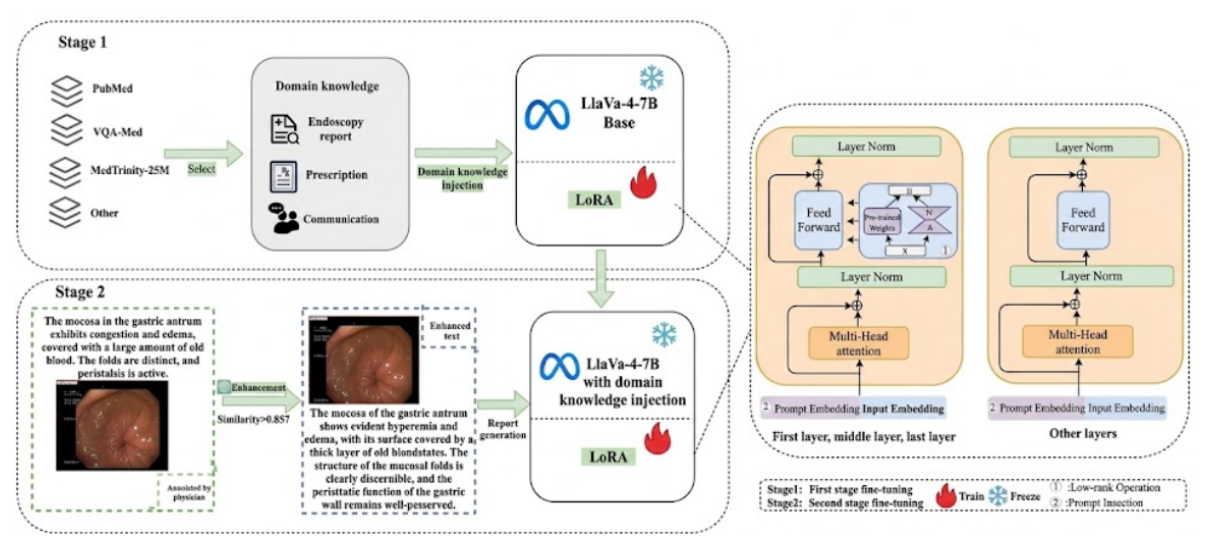
\includegraphics[width=0.85\textwidth]{Fig-1.png}
\caption{Architecture of fine-tuning large language model. Stage 1 and Stage 2 represent the first-stage and second-stage fine-tuning, respectively. The right side shows an expanded diagram of the P-LoRA method. The text highlighted in green is our main work.}
\label{fig:arch}
\end{figure}

\subsection{Two-stage fine-tuning strategy}
General multimodal large language models (MLLMs) exhibit knowledge gaps in endoscopy, particularly in understanding specific lesion characteristics and medical terminology. To address this limitation and improve the quality of generated endoscopic reports, we propose a two-stage fine-tuning strategy [42] that explicitly separates domain knowledge acquisition from report generation. This separation allows the model to first internalize core medical knowledge and then adapt to the stylistic and structural conventions of professional endoscopic reports, leading to more accurate and clinically consistent outputs.
In the first stage, three complementary public datasets are used to provide the model with broad medical domain knowledge before it encounters any institution-specific data.

PubMed [8] has an indexing over 35 million citations and abstracts from life science journals worldwide. We leverage the PubMed Central (PMC) Open Access subset, which provides full-text articles with embedded figure--caption pairs. These image--text pairs are filtered using a curated gastroenterology vocabulary to extract GI-relevant records, covering the esophagus, stomach, duodenum, and colon. The resulting subset provides rich semantic grounding in medical terminology, lesion descriptions, and anatomical expressions, establishing a strong foundation for multimodal pretraining.

MedTrinity-25M [26] is a large-scale multimodal medical dataset comprising approximately 25 million image--text pairs structured as (image, region, enriched description) triplets. It spans multiple imaging modalities and clinical specialities, including radiology (X-ray, CT, MRI), pathology (histology slides), and endoscopy. Each triplet associates a specific image region with a dense, grounded textual description, enabling fine-grained visual--language alignment. Its breadth of clinical content and scale make it particularly valuable for teaching the model diverse visual patterns and associated diagnostic language across medical domains.

VQA-Med [27] originates from the ImageCLEF 2019 medical visual question answering challenge and consists of over 4{,}200 radiology images paired with clinically relevant question--answer pairs. The questions span four categories: modality recognition, plane identification, organ identification, and abnormality detection. By training on VQA-Med, the model develops multimodal reasoning skills — learning to associate visual features with structured clinical questions and precise factual answers. This strengthens the model's ability to interpret diagnostic images in the context of targeted clinical queries, complementing the broader descriptive knowledge acquired from PubMed and MedTrinity-25M.

By leveraging the extensive domain knowledge available in these public datasets for the first-phase fine-tuning, the model can effectively acquire core medical knowledge related to the stomach, including lesion localization, language expressions of structural changes in tissues, and common terms used in diagnostic reports. During this phase, we freeze the vision encoder and other components, performing limited parameter fine-tuning only on the large language model.
In the second stage, to generate templated language that better aligns with the professional style preferences of physicians, we fine-tune the model using data annotated by physicians from Government Medical College, Calicut. After undergoing specific data processing workflows, this phase focuses on fully leveraging the high level of professionalism and standardizing language expressions in the physician-annotated data. By further optimizing the model, it can more accurately learn and master commonly used terminology, sentence structures, and expression patterns in endoscopic reports, thereby enhancing its ability to produce outputs consistent with professional medical documentation practices.



\subsection{P-LoRA method}
Although LoRA has demonstrated good generality across multiple tasks, its fine-tuning performance on domain-specific downstream tasks still requires improvement [11]. To effectively adapt large multimodal models to the endoscopic domain, we combine soft prompt tuning with selective LoRA fine-tuning [42]. Soft prompt tuning is a parameter-efficient technique in which a set of learnable continuous embedding vectors — referred to as soft prompts — are prepended to the model's input sequence. Unlike conventional hard prompts, which consist of manually crafted discrete text tokens, soft prompts are not readable words but rather free-floating vectors in the embedding space that are optimised end-to-end via gradient descent. This allows the model to discover the most effective input-space representations for the target domain without any manual prompt engineering. Soft prompt tuning efficiently guides the model to align with domain-specific language patterns without modifying the majority of model parameters, while LoRA provides targeted weight updates that enhance feature extraction from visual and textual inputs. This combination leverages the strengths of both approaches, achieving better domain adaptation than either method alone: prompt tuning alone may not sufficiently adjust deep representations, whereas LoRA alone may require fine-tuning more parameters and increase computational cost. We apply LoRA selectively to the first, middle, and last layers of the model. This strategy is based on the observation that lower layers capture general visual features, middle layers integrate multimodal interactions, and higher layers encode task-specific representations. By updating only these key layers, we achieve a balance between adaptation performance and computational efficiency, allowing effective domain alignment while keeping training cost manageable as illustrated in Fig. 2.
First, trainable prompt parameters [28] are inserted into each attention layer, as shown in Fig. 2(a). The soft prompt tokens are initialized using the same normal distribution as the pretrained embedding layer. Specifically, a set of special prompt tokens $p = (p_1, p_2, \ldots, p_m)$ with learnable embeddings is added to the front of the input sequence. Let the original input embeddings be $x = (x_1, x_2, \ldots, x_n)$, where each $x_i \in \mathbb{R}^{d_{model}}$ and $d_{model}$ denotes the hidden dimensionality of the model. These prompt tokens are concatenated with the input embeddings to form an extended sequence $x' = (p_1, p_2, \ldots, p_m, x_1, x_2, \ldots, x_n)$, which is then input into the attention layer. During self-attention computation, the query, key, and value are calculated based on this extended sequence, allowing the model to leverage the prompt tokens to capture task-specific information while keeping the output dimensionality consistent with $d_{model}$. No manually crafted prompt content is used; instead, the prompt tokens adapt entirely through task-specific learning. Through this process, the attention layers can better learn representations relevant to the target domain without modifying the pre-trained backbone weights.
Subsequently, LoRA is applied to the feed-forward layers to optimize the model's structural adaptation to the domain. As shown in Fig. 2(b), we combine the use of the LoRA method in the feed-forward layers of the Transformer by inserting low-rank matrices to achieve overall structural optimization, capturing the macro features of the task. To minimize the amount of parameter tuning as much as possible while effectively adapting to the new task, LoRA is applied only to the first layer, middle layers, and the final layer. The goal is to enable the model to quickly adapt to new input features in the first layer, adjust the model's focus on domain-specific information and knowledge expression in the middle layers, and finally optimize the generated output for task-specific needs. Specifically, the input dimension is expanded from $d_{model}$ to a larger dimension $d_{ff}$ in the first fully connected layer, which means inserting a low-rank matrix at the weight matrix of the fully connected layer. The original weight matrix $W \in \mathbb{R}^{m \times n}$ needs to be optimized. In traditional fine-tuning methods, all the parameters in $W$ are updated. However, LoRA proposes a more efficient approach, which is to keep $W$ unchanged and only add a low-rank adjustment term $\Delta W$, such that the fine-tuned weight matrix is as shown in Formula (1).
\begin{equation}
W' = W + \Delta W
\label{eq:lora}
\end{equation}
$\Delta W$ is decomposed into a low-rank form $\Delta W = BA$, where $B \in \mathbb{R}^{m \times r}$, $A \in \mathbb{R}^{r \times n}$, and $r$ is the rank of the decomposition, with the condition that $r \ll \min(m, n)$. These low-rank matrices capture the primary information in the weight matrix, reducing reliance on full-parameter fine-tuning while maintaining efficient representational capacity. Next, the intermediate results undergo a nonlinear transformation using the ReLU activation function, further enhancing the model's expressiveness. In the second fully connected layer, the $d_{ff}$ dimension is mapped back to the original input dimension $d_{model}$. This transformation ensures that the more complex representations obtained after the nonlinear transformation are projected back to the same dimension as the input, maintaining consistency with other parts of the model. The feedforward layer integrates the nonlinear transformations with the contextual information learned by the attention layer, preserving critical context and making the model's overall representation more expressive.
As a result, the feedforward layer and the attention layer form a complementary optimization relationship. The attention layer, through prompt tokens, enhances sensitivity to task-specific information, while the feedforward layer, utilizing LoRA's low-rank decomposition combined with nonlinear transformations, increases the complexity and compactness of the representations. This ensures the model achieves a good balance between task adaptability and efficiency. For the multimodal fine-tuned model, inputting an image $I$ along with a prompt $P$ produces a generated report $Y = (y_1, y_2, \ldots, y_T)$ according to the following autoregressive conditional probability Formula (2).
\begin{equation}
Y = \arg\max \prod_{t=1}^{T} P(y_t \mid y_{<t}, I, P; \theta)
\label{eq:autoregressive}
\end{equation}
where $\theta$ are the model parameters, and $y_{<t}$ denotes all previously generated tokens.

\begin{figure}[ht]
\centering
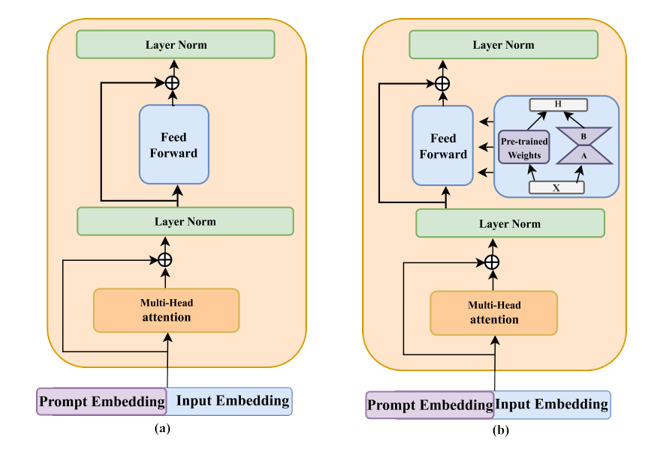
\includegraphics[width=0.85\textwidth]{Fig-2.png}
\caption{P-LoRA method. (b) illustrates the fine-tuning approach used in the first, middle, and final layers, while (a) shows the approach applied to all other layers.}
\label{fig:plora}
\end{figure}

\subsection{Data optimization and filtering}
In this experiment, we use clinical gastroscopy reports collected from Government Medical College, Calicut as the research data. These reports provide detailed records of patients' gastric health, including a large number of gastric endoscopic images that cover key areas such as the esophagus, cardia, fundus, body, antrum, pylorus, duodenal bulb, and descending segment. These images not only provide intuitive visual information for our research but are also crucial for accurately assessing the condition of the stomach. Additionally, the reports include detailed descriptions written by skilled physicians, based on their clinical experience and professional knowledge, providing a thorough record and analysis of gastric. However, some reports may be incomplete, quial or contain awkward or erroneous sentences. Recently, GPT-4 has demonstrated outstanding capabilities in assisting with text processing, providing valuable references for our research [29,30]. Therefore, we leverage GPT-4 to enrich and optimize text sentences.
Templatizing textual sentences helps unify the structure of input data and standardize its formatting, thereby effectively reducing data noise caused by inconsistent expression. For complex medical texts, the application of standardized templates is particularly critical: it ensures that the model focuses on extracting key clinical features during the fine-tuning phase, while avoiding interference from non-uniform descriptive styles across different reports. To implement this templatization, we first provide GPT-4 with a structured positive prompt: You are a professional medical text processing assistant. Your task is to convert the following endoscopic image description sentence into a standardized template format: ``This image shows (gastric region). It describes the following features (details of color, texture, presence)''. To ensure methodological transparency and reproducibility, we explicitly define the interaction protocol. First, raw sentences are provided to GPT-4 with prompts for template conversion. Next, the generated outputs are reviewed by experienced gastroenterologists, who verify medical accuracy, correct terminology usage, and check logical consistency. Finally, low-quality or inconsistent outputs are revised or discarded. Through this multi-step process, GPT-4 serves as an auxiliary tool for annotation, while expert physicians guarantee clinical validity and professional reliability.
During the optimization process, a core principle must always be followed: the optimized sentence must remain semantically consistent with the original sentence, ensuring that the conveyed information is not altered or lost. To this end, introducing a reliable semantic consistency judgment method is crucial. This not only helps assess the semantic alignment between the optimized sentence and the original sentence, providing quality assurance for the optimization process, but also strikes a balance between richness and accuracy in text expression. To ensure that the sentences remain semantically consistent with the original during the optimization process, we introduced a semantic consistency evaluation method based on cosine similarity. Sentence-BERT [31] is used for feature extraction to obtain the vector representations of both the original and optimized sentences. Assume that $u$ is the vector representation of the original sentence, and $v$ is the vector representation of the optimized sentence. Then the resulting similarity value between the original sentence and the optimized sentence is shown in Formula (3).
\begin{equation}
S = \frac{\mathbf{u} \cdot \mathbf{v}}{\|\mathbf{u}\| \|\mathbf{v}\|}
\label{eq:cosine}
\end{equation}
where $S$ denotes the similarity value. In practical applications, we set the similarity threshold to 0.85 and filter all generated sentences one by one based on this criterion. If certain texts fail to meet the set threshold, new sentences are regenerated until the requirement is satisfied, thereby achieving the goal of data enhancement.



\clearpage
\subsection{Data Augmentation}
The private clinical dataset obtained from Government Medical College, Calicut initially comprised approximately 6,500 physician-annotated endoscopic reports. While each report is of high clinical quality, this volume is insufficient for robust fine-tuning of a large multimodal model. To expand the dataset in a clinically valid manner, we apply two complementary augmentation strategies: rotation augmentation and stochastic translation augmentation.

\subsubsection{Rotation Augmentation}
Each original endoscopic image is rotated by $0^\circ$, $90^\circ$, $180^\circ$, and $270^\circ$, producing four variants per image. This is clinically safe because tissue textures and lesion appearances are invariant to rotation in endoscopic imaging. The augmentation produces a structured $4\times$ expansion of the base dataset:
\begin{itemize}
\item Base reports: $6{,}500$
\item After rotation: $6{,}500 \times 4 = 26{,}000$ reports
\end{itemize}
Each report consists of 960 tokens (784 visual tokens + 176 text tokens), so the rotated corpus amounts to $26{,}000 \times 960 = 24{,}960{,}000$ tokens.

\subsubsection{Stochastic Translation Augmentation}
To simulate the natural camera jitter that occurs during real endoscopic examinations, we apply stochastic translation to a subset of the rotated images using a Bernoulli selection process with probability $p = 0.2$. For each selected image, the translation vector $(\tau_x, \tau_y)$ is drawn from a truncated Gaussian distribution:
\[
\tau_x \sim \mathcal{N}(0,\,(0.05W)^2), \quad \text{clamped to } [-0.15W,\, +0.15W]
\]
\[
\tau_y \sim \mathcal{N}(0,\,(0.05H)^2), \quad \text{clamped to } [-0.15H,\, +0.15H]
\]
where $W$ and $H$ are the image width and height respectively. This guarantees that at least 72.25\% of the original image content is preserved, ensuring that diagnostic features remain intact. The translation augmentation adds approximately $26{,}000 \times 0.2 = 5{,}200$ additional reports, contributing $5{,}200 \times 960 = 4{,}992{,}000$ tokens.

\subsubsection{Combined Dataset Size}
The combined token count after both augmentations is:
\[
24{,}960{,}000 + 4{,}992{,}000 \approx 29{,}952{,}000 \text{ tokens} \approx 29.95\text{M tokens}
\]
The final second-stage training set thus comprises approximately $31{,}200$ image--report pairs, which substantially expands the original 6,500 clinical reports while preserving clinical validity. A 5\% held-out validation split (per the training configuration) is applied to this augmented dataset, yielding approximately 29,640 training samples and 1,560 validation samples.

Figure~\ref{fig:augmentation} illustrates representative examples of the two augmentation strategies applied to a sample endoscopic image.

\begin{figure}[ht]
\centering
\begin{minipage}[t]{0.31\textwidth}
    \centering
    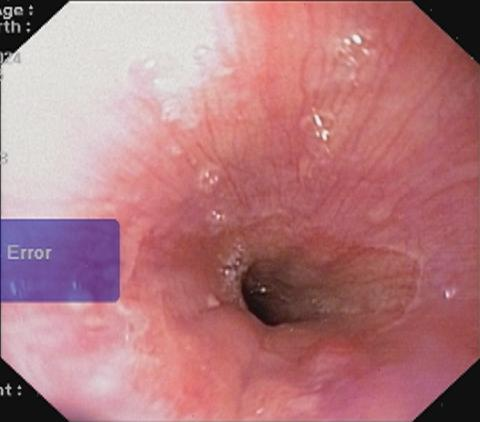
\includegraphics[width=\textwidth]{aug_original.jpg}
    \subcaption{Original}
\end{minipage}\hfill
\begin{minipage}[t]{0.31\textwidth}
    \centering
    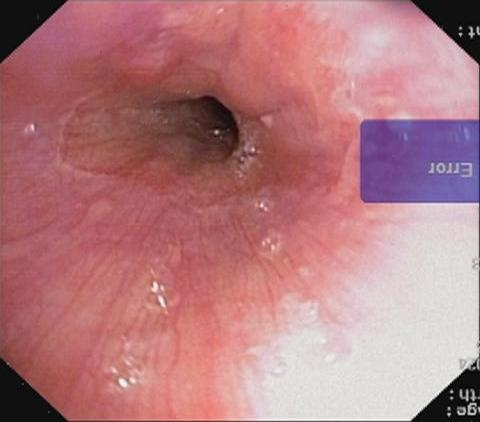
\includegraphics[width=\textwidth]{aug_rotated_90.jpg}
    \subcaption{Rotated (90°)}
\end{minipage}\hfill
\begin{minipage}[t]{0.31\textwidth}
    \centering
    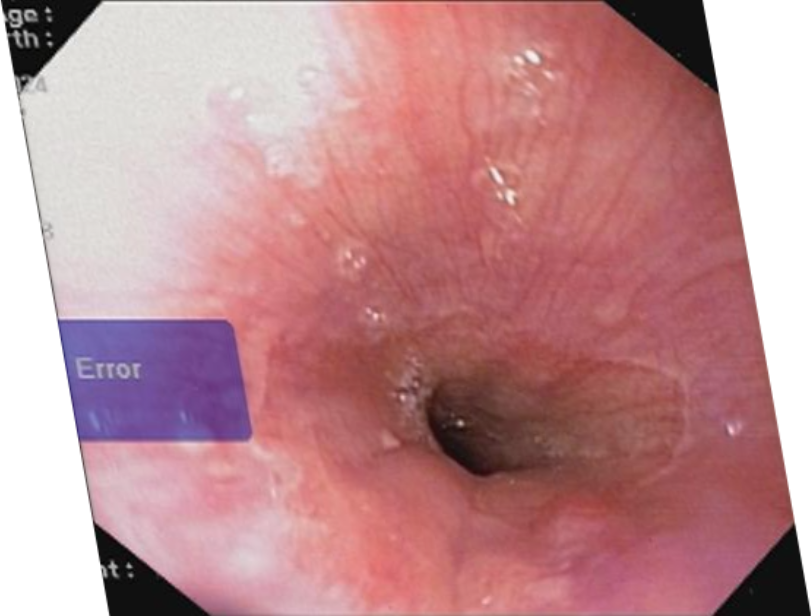
\includegraphics[width=\textwidth]{aug_translated.png}
    \subcaption{Stochastic Translation}
\end{minipage}
\caption{Examples of data augmentation applied to an endoscopic image. (a) Original image from GMC Calicut dataset. (b) Image after 90° rotation — clinically safe as lesion morphology is rotation-invariant in endoscopy. (c) Image after stochastic translation (Bernoulli $p=0.2$, $\sigma=5\%W$) simulating natural camera jitter, with at least 72.25\% overlap guaranteed.}
\label{fig:augmentation}
\end{figure}

\subsection{Chain-of-Thought Integration}
\subsubsection{The Interpretability Problem and Motivation}
A key concern with direct diagnosis generation from endoscopic images is the ``black-box'' nature of the model's reasoning: the model produces a final diagnostic label or report without revealing the intermediate reasoning steps, making the output difficult to trust or verify clinically. To address this, we augment the second-stage training data with chain-of-thought (CoT) reasoning sequences.

\subsubsection{CoT Implementation}
Each training question--answer pair is reformulated to include a step-by-step reasoning chain. The chain forces the model to structure its answer as: \textit{anatomical identification} $\rightarrow$ \textit{visual observation} $\rightarrow$ \textit{diagnosis}. During fine-tuning, the model learns to mimic this transparent reasoning process by predicting the full chain, not just the final conclusion.

For example, contrast the two modes of response:

\medskip
\noindent\textbf{Before CoT (baseline):}
\begin{quote}
\textit{Input:} [Image] ``What is the diagnosis?''\\
\textit{Output:} ``Grade II Esophageal Varices.''
\end{quote}

\noindent\textbf{After CoT (our model):}
\begin{quote}
\textit{Input:} [Image] ``Analyze the image step-by-step and provide a diagnosis.''\\
\textit{Output:}\\
\textbf{Observation 1:} I observe the lower third of the oesophagus.\\
\textbf{Observation 2:} There are swollen, tortuous submucosal veins present.\\
\textbf{Observation 3:} The veins occupy less than one third of the lumen, with no red colour signs.\\
\textbf{Conclusion:} Therefore, the diagnosis is Grade II Esophageal Varices.
\end{quote}
\medskip

\subsubsection{Impact on Clinical Utility}
By training the model to produce explicit reasoning chains, the system transitions from a black-box predictor to an interpretable diagnostic assistant. The key benefits are: (1) clinicians can verify each reasoning step independently; (2) subtle mistakes in intermediate observations become visible and correctable; and (3) the structured output format aligns with the way clinical reports are written, reinforcing the model's professional language generation. This CoT integration is particularly valuable in real-world deployment where clinical trust and accountability are paramount.

\chapter{Results}
\section{Experiments and discussion}
To validate the effectiveness of our proposed method, we conducted fine-tuning on both public and private datasets and evaluated the results across automated metrics and expert physician evaluation.

\subsection{Datasets}
We adopt a two-phase fine-tuning approach, where the first phase screens gastrointestinal descriptive data from open-source medical datasets, as shown in Table~\ref{tab:data-distribution}. At this stage, we use a gastroenterology medical vocabulary as the basis to conduct comprehensive screening and precise filtering of the data, ensuring that the final dataset centers on core knowledge in the field of gastroenterology. Irrelevant information is effectively removed, achieving a high degree of alignment between the dataset content and the target domain. After the initial screening process, each report is independently reviewed by experienced gastroenterologists, who filter out low-quality or unusable samples, further enhancing the dataset's professional reliability and clinical applicability. These datasets, including PubMed, encompass rich content across general medicine, providing detailed descriptions of various body parts and diseases. With their large scale and comprehensive semantic knowledge, these datasets are valuable resources for medical research and model training. By filtering and cleaning high-relevance gastrointestinal data from PubMed [6], MedTrinity-25M [12], and VQA-Med [6], we obtained a subset of approximately 60K records for the first phase of fine-tuning. This dataset not only includes detailed problem descriptions but also contains extensive domain knowledge, enabling the model to learn foundational semantic knowledge, lesion descriptions, and anatomical expressions related to gastrointestinal medicine, thereby laying a solid groundwork for subsequent training.
In the second stage, we use gastroscopy reports collected from Government Medical College, Calicut as research data. These reports are strictly screened and processed using the method described in Section 4.1.4, resulting in a more targeted training dataset. The data are derived from real clinical patients and have undergone a rigorous automated de-identification pipeline to ensure compliance with India's Digital Personal Data Protection (DPDP) Act and HIPAA-like privacy guidelines. The de-identification process irreversibly removes all Protected Health Information (PHI) from both the textual reports and associated metadata, including patient identifiers (name, patient ID), age and gender fields, visit dates, and procedure-specific numbers (UGI-OGD report numbers). This ensures that no patient-identifiable information is retained in the training corpus, and the process is irreversible by design to prevent re-identification. Figure~\ref{fig:deidentification} shows the automated de-identification pipeline applied to a representative patient report header.

\begin{figure}[ht]
\centering
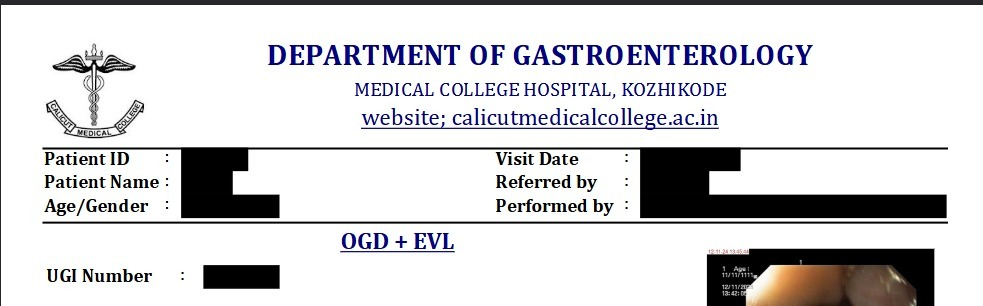
\includegraphics[width=0.85\textwidth]{deidentification_diagram.jpeg}
\caption{Automated de-identification pipeline applied to GMC Calicut endoscopic reports. All Protected Health Information (PHI) fields — including Patient ID, Name, Age/Gender, Visit Date, and UGI-OGD report numbers — are irreversibly redacted prior to entering the training pipeline, in compliance with the DPDP Act.}
\label{fig:deidentification}
\end{figure}

In the constructed dataset, normal samples account for approximately 40\%, while abnormal samples make up about 60\%, ensuring sufficient representation of pathological cases for the model to learn discriminative features. The abnormal samples encompass a variety of gastrointestinal conditions, including esophageal varices, gastric polyps, gastric bleeding, gastric ulcers, early-stage gastric cancer, and advanced gastric cancer, demonstrating a high diversity of disease types. The images are collected from multiple key anatomical regions of the gastrointestinal tract, such as the esophagus, cardia, fundus, body, antrum, pylorus, as well as the duodenal bulb and descending segment, ensuring the dataset's comprehensiveness and representativeness. These images are all selected by endoscopists from the key anatomical regions during actual clinical examinations. All images are captured using different endoscopic devices at Government Medical College, Calicut, but uniformly configured to the same resolution of $1920 \times 1080$. Although the raw images are captured at $1920\times1080$ pixels, they are resized to $336\times336$ during preprocessing as input to the CLIP-ViT-L/14 vision encoder. The dataset uses a 5\% validation split (per the training configuration), with the remaining data used for training. A separate held-out test set is used for final evaluation. Due to the standardized collection process, all images meet clinical diagnostic requirements in terms of clarity, key region coverage, validity, and lesion feature presentation. Considering that the optimization process may introduce non-standard expressions or inconsistent terminology even when semantic changes are minimal, multiple experienced physicians rigorously review the optimized reports to ensure medical professionalism and the accurate use of terminology. They also make necessary revisions to any parts that exhibit deviations.
All data meet the predefined similarity threshold, with the vast majority achieving a similarity score above 0.9 (78.6\%), indicating that the data quality is highly satisfactory. The filtered dataset contains approximately 6,500 high-quality physician-annotated reports from Government Medical College, Calicut. These reports exhibit a high degree of professionalism in language expression, showcasing the terminology, sentence structures, and diagnostic habits commonly used by physicians when writing endoscopic reports, which effectively enhance the model's generative capabilities in the professional domain. Compared to publicly available data, the amount of data in the second stage is relatively small, but it focuses on high professionalism and standardized language expression, concentrating on the precise description of endoscopic images and the documentation of lesion information.

\begin{table}[ht]
\centering
\caption{Data distribution of the first and second stage. We list the different datasets used in the first and second stages, including source, type, number, and description.}
\label{tab:data-distribution}
\renewcommand{\arraystretch}{1.2}
\begin{tabular}{p{1.5cm}p{2.5cm}p{2.5cm}p{1.2cm}p{5.5cm}}
\toprule
Stage & Data source & Data type & Number & Description \\
\midrule
First stage & PubMed; MedTrinity-25M; VQA-Med & Gastrointestinal tract related knowledge & 60k & Descriptive data related to the gastrointestinal tract, selected from open medical datasets. Includes fundamental semantic knowledge, lesion descriptions, and anatomical expressions. \\
Second stage & Physician-annotated data from Government Medical College, Calicut & Specialized endoscopic report data & 6.5k (base); $\sim$31k (after augmentation) & High-quality, professional endoscopic report data, cleaned and optimized for generating template-based language matching physicians' professional style. Expanded via rotation and stochastic translation augmentation. \\
\bottomrule
\end{tabular}
\end{table}

\subsection{Implementation details}
We conduct fine-tuning experiments based on the LLaVA-4 base model, using the P-LoRA method for fine-tuning in both the first and second stages. The fine-tuning settings for both stages are configured as rank = 64, $\alpha$ = 32, and dropout = 0.05. The micro-batch size for both stages is set to 2, with gradient accumulation steps set to 4, yielding an effective global batch size of 8. The initial learning rate is configured to 2e-4, the warm-up ratio is set to 0.1, and the maximum sequence length is 4096. The model is trained for 4 epochs using the AdamW optimizer with 8-bit quantization (adamw\_bnb\_8bit), a cosine learning rate scheduler, and bfloat16 (BF16) precision. Flash Attention 2 is enabled for memory-efficient attention computation. The seed is set to 42. During testing, the temperature is set to 0, while both top\_p and top\_k are set to None, as shown in Table 2.

\begin{description}
    \item[Vision Encoder] CLIP-ViT-L/14. Pre-trained on 400M pairs; robust medical visual features; L size balances capacity vs. speed; 14×14 patch grid captures both anatomy and small lesions.
    \item[Image resolution] 336×336 pixels. Standard for LLaVA; sufficient detail without excessive memory.
    \item[Patch size] 14×14 (24×24 grid).
    \item[Total vision tokens] 577 per image (576 patches + CLS). Each patch token carries localised information, enabling the language model to “see” global and local structures.
    \item[Training Precision] bfloat16 (BF16). Halves memory vs. FP32, no performance loss.
    \item[Attention] Flash Attention 2. Memory-efficient exact attention; 5--10$\times$ VRAM reduction for long sequences.
\end{description}

Our tests are conducted on a Linux system using the PyTorch platform. The system is powered by two Intel(R) Xeon(R) 6505P processors (12 cores per socket, 2 sockets, 48 threads total), 251 GiB RAM, and one NVIDIA H200 NVL GPU (143 GB HBM3e, CUDA 13.0). The Python version in use is 3.12.3 with PyTorch 2.11.0+cu130. The trainable parameters introduced by our P-LoRA method account for approximately 0.343\% of the full model size. The actual GPU memory usage during training is approximately 43 GB, and the average inference time per report is around 7 s.

\begin{table}[H]
\centering
\caption{Hyperparameter settings.}
\label{tab:hyperparams}
\begin{tabular}{lcc}
\toprule
Hyperparameter & Stage 1 & Stage 2 \\
\midrule
Learning rate & 2e-4 & 2e-4 \\
Batch size & 2 & 2 \\
Gradient accumulation & 4 & 4 \\
Optimizer & AdamW-8bit & AdamW-8bit \\
Warm-up ratio & 0.1 & 0.1 \\
Max sequence length & 4096 & 4096 \\
LoRA rank & 64 & 64 \\
$\alpha$ & 32 & 32 \\
Dropout & 0.05 & 0.05 \\
Prompt tokens & 64 & 64 \\
Num epochs & 4 & 4 \\
Random seed & 42 & 42 \\
\bottomrule
\end{tabular}
\end{table}

\subsection{Evaluation metrics}
A large number of previous studies [32--34] adopt metrics such as CIDEr, ROUGE, and METEOR to evaluate the similarity between generated medical descriptions and the original descriptions. CIDEr (Consensus-based Image Description Evaluation) [35] is specifically designed for image description tasks. CIDEr aligns more closely with human judgment when determining the similarity between two sentences because it employs TF-IDF to assign different weights to various n-grams. Intuitively, frequently occurring phrases are given lower weights, while less common phrases are considered more distinctive, drawing more attention from people to these unique words.
ROUGE (Recall-Oriented Understudy for Gisting Evaluation) [36] is a metric used for automatically evaluating the quality of generated text. It is commonly applied in tasks such as summarization, machine translation, and text generation. ROUGE assesses the quality of generated text by measuring the overlap between the generated and reference texts, with a primary focus on recall.
METEOR (Metric for Evaluation of Translation with Explicit Ordering) [37] is a metric used to evaluate the quality of text outputs in tasks such as machine translation, image caption generation, and other natural language generation tasks. It is based on precise matching and semantic similarity between sentences, addressing shortcomings of traditional metrics like BLEU [38], which are less sensitive to word order and semantic similarities.
However, these metrics mainly focus on linguistic form and are limited in capturing the clinical correctness and practical utility of the reports. Therefore, to further assess the clinical validity and quality of the generated reports, we introduce expert human evaluation.

\subsection{Experimental results}
\subsubsection{Comparison of different models}
In this section, to demonstrate the effectiveness of our method, we select several mainstream large models for comparison, including Qwen2-VL-7B-Instruct, BLIP-2 (opt-2.7b), and InstructBLIP, and conduct a comprehensive comparative analysis with our method, as shown in Table 3. To better evaluate experimental performance, we test the models using the same prompt as our model: ``Observe this endoscopic image and describe the gastric features presented in the image''.
Unlike the aforementioned models, Our Model is fine-tuned on a strong foundation model to adapt it specifically to the professional task of endoscopic report generation. On the one hand, the proposed two-stage fine-tuning strategy enables the model to progressively evolve from learning endoscopic medical knowledge to generating specialized and standardized clinical reports. On the other hand, the task-oriented design and the fine-tuning strategy tailored for endoscopic image--report generation significantly enhance the model's domain adaptability. In addition, the construction of high-quality and professionally annotated endoscopic report data is an indispensable component of this work.

\begin{table}[ht]
\centering
\caption{Comparison of different models. We compare our experimental results with existing influential multimodal large models, with key metrics including CIDEr, ROUGE-L, METEOR, BLEU-4, and BERTScore.}
\label{tab:model-comparison}
\resizebox{\textwidth}{!}{%
\begin{tabular}{lccccc}
\toprule
Method & CIDEr $\uparrow$ & ROUGE-L $\uparrow$ & METEOR $\uparrow$ & BLEU-4 $\uparrow$ & BERTScore $\uparrow$ \\
\midrule
Qwen2-VL-7B-Instruct & 0.0078 & 0.0504 & 0.0564 & 0.0009 & 0.8317 \\
BLIP-2 & 0.0079 & 0.0147 & 0.0347 & 0.0002 & 0.7957 \\
InstructBLIP & 0.0088 & 0.0320 & 0.0583 & 0.0004 & 0.8196 \\
\textbf{Our Model} & \textbf{0.0531} & \textbf{0.2632} & \textbf{0.1187} & \textbf{0.0006} & \textbf{0.8760} \\
\bottomrule
\end{tabular}%
}
\end{table}

\subsubsection{Evaluation of the accuracy and quality of generated reports}
To assess the clinical accuracy and practical usability of the generated endoscopic reports, we conduct a structured physician-based evaluation. Two senior endoscopists (each with more than 10 years of clinical experience in gastrointestinal endoscopy) from Government Medical College, Calicut are invited as expert reviewers. Both reviewers participate voluntarily and independently, and they are blinded to the model identity and experimental settings to avoid potential bias. Each endoscopist independently evaluates the generated reports based solely on the corresponding endoscopic images, without access to reference reports or each other's judgments. Report accuracy is assessed based on whether all content in the report aligns with actual medical facts. Reports are marked as ``Correct'' if all content is accurate, and ``Incorrect'' if any factual error or clinically inconsistent description is present. In cases of disagreement between the two experts, a joint discussion is conducted to reach a consensus label.
The expert physicians also noted that MVLMERG generates reports approximately 5--7 s per image, compared to the 3--5 min typically required for manual report writing, significantly reducing workload and allowing clinicians to focus on diagnosis and patient communication.

\chapter{Conclusion and Future work}
\section{Limitations and future work}
For example, achieving more precise automatic detection of lesion locations, improving the accuracy of gastric cancer grading and classification, and optimizing the recognition and diagnosis of complex lesions remain significant challenges.
Although our model demonstrates high accuracy in generating endoscopic reports, errors of varying clinical severity can occur. High-severity errors include omissions of critical findings, such as early-stage gastric cancer or active bleeding, which may directly impact diagnosis and treatment decisions. Low-severity errors primarily involve minor wording or stylistic inconsistencies that do not significantly affect clinical interpretation. Expert review shows that most errors fall into the low-severity category, while high-severity errors are relatively rare but require particular attention to ensure patient safety. These findings emphasize the need for qualified clinicians to review all model-generated reports and highlight the importance of careful integration of AI tools into clinical workflows. Although the endoscopic equipment at Government Medical College, Calicut covers multiple brands, the same brand may differ across hospitals, and variations in physicians' expertise may also lead to differences in reports. This single-centre data source may restrict the model's generalizability across different hospitals and clinical environments. In practice, variations in endoscopic imaging equipment, illumination conditions, and color calibration between hospitals can alter image characteristics, while differences in reporting styles, terminology, and diagnostic criteria among physicians may lead to textual inconsistencies. Such physician dependent annotation styles may introduce implicit bias during training, potentially affecting the phrasing, emphasis, or level of diagnostic certainty in the generated reports. Furthermore, regional differences in disease prevalence and case complexity may introduce additional bias. These factors can cause domain shifts that reduce the model's performance when applied to unseen data. If endoscopic images present ambiguous or contradictory visual cues, the model is designed to generate conservative, evidence-based descriptions rather than definitive diagnoses. This approach helps prevent over-interpretation and maintains clinical reliability. In addition, automatically flagging instances with high uncertainty for closer physician review represents a highly valuable direction for future work.
Future work will involve a concrete multi-center validation plan. Specifically, we plan to collaborate with several hospitals in different regions of India to collect diverse endoscopic image--report pairs from various imaging systems and patient populations. The evaluation will include cross-hospital transfer tests, consistency assessments across different endoscopic brands, and clinical validation by independent physicians. This study primarily focuses on the analysis of individual endoscopic images, where diagnostic conclusions are limited to describing specific lesions observed within each image. However, in real-world clinical practice, endoscopists typically acquire multiple images per patient to form a comprehensive diagnostic assessment. Accordingly, an important direction for future work is to extend the current single-image interpretation framework toward multi-image and patient-level report generation, enabling integrated diagnostic summaries that more closely reflect actual clinical workflows. Building upon this direction, future research will further explore video-based endoscopy analysis by modeling temporal information across consecutive frames. Such temporal modeling has the potential to support more robust lesion localization, progression analysis, and comprehensive patient-level diagnosis. Additionally, regional differences in medical practices and terminology may lead to interpretative biases in the generated medical descriptions. When deploying the proposed model in new hospitals or clinical settings, domain shifts may arise due to differences in endoscopic devices, imaging protocols, patient populations, and report-writing styles. To address this issue, several lightweight adaptation strategies can be adopted. First, parameter-efficient fine-tuning methods can be applied using a small number of locally collected image--report pairs, enabling rapid domain adaptation with limited computational cost. Second, prompt adjustment provides a flexible alternative, where hospital-specific reporting templates, terminology preferences, or anatomical naming conventions can be incorporated into structured prompts without updating model parameters. In addition, continuous feedback from clinicians can be used to iteratively refine prompts or select representative samples for incremental fine-tuning. These strategies allow the model to be efficiently adapted to new hospitals while preserving data privacy and minimizing deployment overhead.
Regarding the application of large language models in healthcare, the foremost challenge lies in data availability. Collecting endoscopic data is time-consuming and costly, so it is important to explore how LLM-based approaches can generate synthetic data that closely reflect real clinical scenarios while adhering to ethical standards [40,41]. Furthermore, in terms of LLM architecture, an important future direction is to design models that effectively leverage the strengths of both language and visual encoders, achieving efficient multimodal feature fusion. Research on clinical endoscopy videos also holds greater practical significance and applicability. Finally, direct inference with LLMs may not fully exploit their potential; existing strategies such as rethinking or chain-of-thought reasoning may enhance their reasoning capabilities, representing another highly valuable direction for future work. We are actively communicating with Government Medical College, Calicut, to seek approval for two concurrent goals: expanding the dataset with additional physician-annotated endoscopic cases and releasing a de-identified subset for the broader research community. A larger and more diverse clinical dataset would directly improve model generalizability, reduce domain bias, and enable finer-grained classification of gastric and oesophageal conditions. Both data expansion and public release are subject to institutional review and privacy regulations under India's Digital Personal Data Protection (DPDP) Act, and we are committed to making as much data as ethically permissible accessible to support further research in automated endoscopic report generation. In addition, the pretrained model, P-LoRA configurations, and training scripts will be made available upon publication to support reproducibility and further research.
To enable practical clinical deployment, we plan to explore model quantization strategies to reduce memory footprint while preserving inference quality. A RESTful API layer and electronic health record (EHR) integration module are planned to facilitate seamless adoption into existing clinical workflows. Full clinical deployment is contingent on formal approval from the Institutional Ethics Committee (IEC) of Government Medical College, Calicut, and compliance with applicable regulatory standards.

\begin{figure}[ht]
\centering

\includegraphics[width=0.85\textwidth]{Fig-10.png}
\caption{Workflow of MVLMERG in clinical practice, including endoscopic image input, MVLMERG-generated draft report, physician review and editing, and final integration into the EMR system.}
\label{fig:workflow}
\end{figure}

\section{Conclusion}
In this study, we develop an endoscopic image interpretation model using a prompt-based LoRA fine-tuning method, aiming to fully explore and utilize the potential of existing multimodal foundational models to achieve precise medical image interpretation through a two-stage fine-tuning strategy [42].
After fine-tuning, the model shows remarkable performance in generating descriptions of endoscopic images, with particularly high sensitivity to recognizing image morphological features. In the task of interpreting endoscopic reports, our model significantly outperforms models such as GPT-4V and HuatuoGPT-Vision-7B.

\section*{CRediT authorship contribution statement}
Praval Pattam: Software, Writing -- original draft, Methodology, Conceptualization. Theenesh Potluri: Software, Writing -- review \& editing, Validation, Formal analysis. Pranav Sai Sarvepalli: Software, Data curation, Investigation.

\section*{Ethics and safety}
All procedures in this study comply with ethical standards for medical data usage. The dataset used for model training and evaluation is fully de-identified by the data-providing institution, with all Protected Health Information (PHI) removed in accordance with HIPAA-like privacy guidelines. No patient-identifiable information is accessed or processed during the development of this study.
To ensure safe deployment, all model-generated outputs are intended solely for research purposes. The system is not designed for direct clinical application, and any generated report is required to undergo review and verification by licensed physicians before being used in clinical decision-making. In addition, all experiments are approved by the corresponding institutional ethics committee, and data usage strictly follows the institution's data governance requirements.

\section*{Ethics statements}
This study was conducted in accordance with the ethical guidelines of Government Medical College, Calicut, and the National Institute of Technology Calicut. All data used in this research were handled with strict confidentiality and used solely for academic purposes.

\section*{Declaration of competing interest}
The authors declare that they have no known competing financial interests or personal relationships that could have appeared to influence the work reported in this paper.

\section*{Data availability}
The authors do not have permission to share data.

\addcontentsline{toc}{chapter}{References}
\begin{thebibliography}{99}
\bibitem{ref1} X. Zhang, X. Zheng, M. Dong, M. Zhang, An endoscopic images and diagnostic records based multimodal method for severity grading of gastric cancer, Biomed. Signal Process. Control. 109 (2025) 107891, \url{http://dx.doi.org/10.1016/j.bspc.2025.107891}.
\bibitem{ref2} X. Chen, X. Zheng, Z. Li, M. Ma, M. Zhang, Self-supervised visual--textual prompt learning for few-shot grading of gastric intestinal metaplasia, Knowl.-Based Syst. 301 (2024) 112303, \url{http://dx.doi.org/10.1016/j.knosys.2024.112303}.
\bibitem{ref3} Y. Okagawa, S. Abe, M. Yamada, I. Oda, Y. Saito, Artificial intelligence in endoscopy, Dig. Dis. Sci. 67 (5) (2022) 1553--1572, \url{http://dx.doi.org/10.1007/s10620-021-07086-z}.
\bibitem{ref4} F. Chadebecq, L.B. Lovat, D. Stoyanov, Artificial intelligence and automation in endoscopy and surgery, Nat. Rev. Gastroenterol. Hepatol. 20 (3) (2023) 171--182, \url{http://dx.doi.org/10.1038/s41575-022-00701-y}.
\bibitem{ref5} C. Krai\v{s}nikovi\'c, R. Harb, M. Plass, W.A. Zoughbi, A. Holzinger, H. M\"uller, Fine-tuning language model embeddings to reveal domain knowledge: An explainable artificial intelligence perspective on medical decision making, Eng. Appl. Artif. Intell. 139 (2025) 109561, \url{http://dx.doi.org/10.1016/j.engappai.2024.109561}.
\bibitem{ref7} X. Zhang, C. Wu, Z. Zhao, W. Lin, Y. Zhang, Y. Wang, W. Xie, Pmc-vqa: Visual instruction tuning for medical visual question answering, 2023, arXiv preprint arXiv:2305.10415. URL \url{https://arxiv.org/abs/2305.10415}.
\bibitem{ref8} C. Li, C. Wong, S. Zhang, N. Usuyama, H. Liu, J. Yang, T. Naumann, H. Poon, J. Gao, LLaVA-med: training a large language-and-vision assistant for biomedicine in one day, in: Proceedings of the 37th International Conference on Neural Information Processing Systems, 2023, p. 24, doi: \url{https://dl.acm.org/doi/10.5555/3666122.3667362}.
\bibitem{ref9} J. White, PubMed 2.0, Med. Ref. Serv. Q. 39 (4) (2020) 382--387, \url{http://dx.doi.org/10.1080/02763869.2020.1826228}.
\bibitem{ref13} Z. Fu, H. Yang, A.M.-C. So, W. Lam, L. Bing, N. Collier, On the effectiveness of parameter-efficient fine-tuning. 37, 11, 2023, pp. 12799--12807, \url{http://dx.doi.org/10.1609/aaai.v37i11.26505}.
\bibitem{ref14} E.J. Hu, Y. Shen, P. Wallis, Z. Allen-Zhu, Y. Li, S. Wang, L. Wang, W. Chen, Lora: Low-rank adaptation of large language models, ICLR 1 (2) (2022) 3, URL \url{https://openreview.net/forum?id=nZeVKeeFYf9}.
\bibitem{ref15} Y. Mao, Y. Ge, Y. Fan, W. Xu, Y. Mi, Z. Hu, Y. Gao, A survey on lora of large language models, Front. Comput. Sci. 19 (7) (2025) 197605, \url{http://dx.doi.org/10.1007/s11704-024-40663-9}.
\bibitem{ref16} S.-W. Pi, M.-S. Park, B.-D. Lee, Enhancing radiology report interpretation with large-scale language models: A two-stage fine-tuning approach, in: 2025 27th International Conference on Advanced Communications Technology, ICACT, 2025, pp. 383--388, \url{http://dx.doi.org/10.23919/ICACT63878.2025.10936299}.
\bibitem{ref17} W. Wang, Q. Lv, W. Yu, W. Hong, J. Qi, Y. Wang, J. Ji, Z. Yang, L. Zhao, X. Song, et al., Cogvlm: Visual expert for pretrained language models, 2024, pp. 121475--121499, 37, arXiv preprint arXiv:2311.03079.
\bibitem{ref18} J. Bai, S. Bai, S. Yang, S. Wang, S. Tan, P. Wang, J. Lin, C. Zhou, J. Zhou, Qwen-vl: A frontier large vision-language model with versatile abilities, 2023, arXiv:2308.12966.
\bibitem{ref19} H. Liu, C. Li, Q. Wu, Y.J. Lee, Visual instruction tuning, in: Proceedings of the 37th International Conference on Neural Information Processing Systems, NIPS '23, Curran Associates Inc, Red Hook, NY, USA, 2023, URL \url{https://dl.acm.org/doi/10.5555/3666122.3667638}.
\bibitem{ref21} J. Chen, C. Gui, R. Ouyang, A. Gao, S. Chen, G.H. Chen, X. Wang, R. Zhang, Z. Cai, K. Ji, et al., Huatuogpt-vision, towards injecting medical visual knowledge into multimodal llms at scale, 2024, arXiv:2406.19280.
\bibitem{ref22} L. Seenivasan, M. Islam, G. Kannan, H. Ren, SurgicalGPT: end-to-end language-vision GPT for visual question answering in surgery, in: International Conference on Medical Image Computing and Computer-Assisted Intervention, 2023, pp. 281--290, \url{http://dx.doi.org/10.1007/978-3-031-43996-4_27}.
\bibitem{ref23} G.-P. Ji, J. Liu, P. Xu, N. Barnes, F.S. Khan, S. Khan, D.-P. Fan, Frontiers in intelligent colonoscopy, 2024, arXiv:2410.17241.
\bibitem{ref24} S. Schmidgall, J. Cho, C. Zakka, W. Hiesinger, Gp-vls: A general-purpose vision language model for surgery, 2024, arXiv:2407.19305.
\bibitem{ref25} H. Xiong, S. Wang, Y. Zhu, Z. Zhao, Y. Liu, L. Huang, Q. Wang, D. Shen, Doctorglm: Fine-tuning your chinese doctor is not a herculean task, 2023, arXiv:2304.01097.
\bibitem{ref26} A.P. Gema, P. Minervini, L. Daines, T. Hope, B. Alex, Parameter-efficient fine-tuning of llama for the clinical domain, 2023, arXiv:2307.03042.
\bibitem{ref27} G. Liu, J. He, P. Li, G. He, Z. Chen, S. Zhong, Pefomed: Parameter efficient fine-tuning of multimodal large language models for medical imaging, 2024, arXiv:2401.02797.
\bibitem{ref28} J. Chen, D. Yang, Y. Jiang, Y. Lei, L. Zhang, MISS: A generative pre-training and fine-tuning approach for med-VQA, in: International Conference on Artificial Neural Networks, Springer, 2024, pp. 299--313, \url{http://dx.doi.org/10.1007/978-3-031-72353-7_22}.
\bibitem{ref29} Y. Lu, S. Hong, Y. Shah, P. Xu, Effectively fine-tune to improve large multi-modal models for radiology report generation, in: Deep Generative Models for Health Workshop NeurIPS 2023, 2023, URL \url{https://openreview.net/forum?id=QAruOR4nUa}.
\bibitem{ref30} X. Wu, R. Xu, P. Wei, W. Qin, P. Huang, Z. Li, L. Luo, Pathinsight: Instruction tuning of multimodal datasets and models for intelligence assisted diagnosis in histopathology, 2024, arXiv:2408.07037.
\bibitem{ref33} Y. Xie, C. Zhou, L. Gao, J. Wu, X. Li, H.-Y. Zhou, S. Liu, L. Xing, J. Zou, C. Xie, Y. Zhou, MedTrinity-25m: A large-scale multimodal dataset with multigranular annotations for medicine, in: The Thirteenth International Conference on Learning Representations, 2025, URL \url{https://openreview.net/forum?id=IwgmgidYPS}.
\bibitem{ref34} A. Ben Abacha, S.A. Hasan, V.V. Datla, D. Demner-Fushman, H. M\"uller, Vqa-med: Overview of the medical visual question answering task at imageclef 2019, in: Proceedings of CLEF (Conference and Labs of the Evaluation Forum) 2019 Working Notes, 2019, URL \url{https://arodes.hes-so.ch/record/4214?v=pdf}.
\bibitem{ref35} X. Liu, K. Ji, Y. Fu, W. Tam, Z. Du, Z. Yang, J. Tang, P-tuning: Prompt tuning can be comparable to fine-tuning across scales and tasks, in: S. Muresan, P. Nakov, A. Villavicencio (Eds.), Proceedings of the 60th Annual Meeting of the Association for Computational Linguistics (Volume 2: Short Papers), Association for Computational Linguistics, Dublin, Ireland, 2022, pp. 61--68, \url{http://dx.doi.org/10.18653/v1/2022.acl-short.8}.
\bibitem{ref36} X. Xiao, Y. Li, X. He, J. Fang, Z. Yan, C. Xie, An assessment framework of higher-order thinking skills based on fine-tuned large language models, Expert Syst. Appl. 272 (2025) 126531, \url{http://dx.doi.org/10.1016/j.eswa.2025.126531}.
\bibitem{ref37} S. Li, W. Tan, C. Zhang, J. Li, H. Ren, Y. Guo, J. Jia, Y. Liu, X. Pan, J. Guo, W. Meng, Z. He, Taming large language models to implement diagnosis and evaluating the generation of LLMs at the semantic similarity level in acupuncture and moxibustion, Expert Syst. Appl. 264 (2025) 125920, \url{http://dx.doi.org/10.1016/j.eswa.2024.125920}.
\bibitem{ref38} N. Reimers, I. Gurevych, Sentence-BERT: Sentence embeddings using siamese BERT-networks, in: Proceedings of the 2019 Conference on Empirical Methods in Natural Language Processing and the 9th International Joint Conference on Natural Language Processing, EMNLP-IJCNLP, 2019, pp. 3982--3992, \url{http://dx.doi.org/10.18653/v1/D19-1410}.
\bibitem{ref39} D.-R. Beddiar, M. Oussalah, T. Sepp\"anen, Automatic captioning for medical imaging (MIC): a rapid review of literature, Artif. Intell. Rev. 56 (5) (2023) 4019--4076, \url{http://dx.doi.org/10.1007/s10462-022-10270-w}.
\bibitem{ref40} A. Zhang, E. Zhao, R. Wang, X. Zhang, J. Wang, E. Chen, Multimodal large language models for medical image diagnosis: Challenges and opportunities, J. Biomed. Inform. 169 (2025) 104895, \url{http://dx.doi.org/10.1016/j.jbi.2025.104895}.
\bibitem{ref41} H. Park, K. Kim, S. Park, J. Choi, Medical image captioning model to convey more details: methodological comparison of feature difference generation, IEEE Access 9 (2021) 150560--150568, \url{http://dx.doi.org/10.1109/ACCESS.2021.3124564}.
\bibitem{ref42} R. Vedantam, C.L. Zitnick, D. Parikh, CIDEr: Consensus-based image description evaluation, in: 2015 IEEE Conference on Computer Vision and Pattern Recognition, CVPR, 2015, pp. 4566--4575, \url{http://dx.doi.org/10.1109/CVPR.2015.7299087}.
\bibitem{ref43} C.-Y. Lin, Rouge: A package for automatic evaluation of summaries, in: Text Summarization Branches Out, 2004, pp. 74--81, URL \url{https://aclanthology.org/W04-1013/}.
\bibitem{ref44} S. Banerjee, A. Lavie, METEOR: An automatic metric for MT evaluation with improved correlation with human judgments, in: Proceedings of the Acl Workshop on Intrinsic and Extrinsic Evaluation Measures for Machine Translation and/Or Summarization, 2005, pp. 65--72, URL \url{https://aclanthology.org/W05-0909/}.
\bibitem{ref45} K. Papineni, S. Roukos, T. Ward, W.-J. Zhu, Bleu: a method for automatic evaluation of machine translation, in: Proceedings of the 40th Annual Meeting of the Association for Computational Linguistics, 2002, pp. 311--318, \url{http://dx.doi.org/10.3115/1073083.1073135}.
\bibitem{ref46} H. Liu, C. Li, Y. Li, Y.J. Lee, Improved baselines with visual instruction tuning, in: 2024 IEEE/CVF Conference on Computer Vision and Pattern Recognition, CVPR, 2024, pp. 26286--26296, \url{http://dx.doi.org/10.1109/CVPR52733.2024.02484}.
\bibitem{ref51} {National Academies of Sciences, Engineering, and Medicine}, Reducing Administrative Burden in Health Care: Strategies to Improve Clinician Well-Being, The National Academies Press, Washington, DC, 2024, \url{https://www.ncbi.nlm.nih.gov/books/NBK608542/}.
\bibitem{ref52} T.D. Shanafelt, C.P. West, L.N. Dyrbye, H. Wang, C. Sinsky, M. Trockel, Changes in burnout and satisfaction with work-life integration in physicians and the general US working population between 2011 and 2020, Mayo Clin. Proc. 97 (3) (2022) 491--506, \url{http://dx.doi.org/10.1016/j.mayocp.2021.11.021}.
\bibitem{ZHANG2026109737} X. Zhang, X. Zheng, Z. Li, M. Ma, X. Liang, X. Ren, M. Zhang, A fine-tuning multimodal large language model for endoscopic report generation, Biomed. Signal Process. Control 118 (2026) 109737, \url{https://doi.org/10.1016/j.bspc.2026.109737}.
\end{thebibliography}
\end{document}
